\documentclass[11pt,a4paper]{article}

\usepackage[utf8]{inputenc}
\usepackage[T1]{fontenc}
\usepackage{graphicx}
\usepackage{amsmath}
\usepackage{booktabs}
\usepackage{geometry}
\usepackage{float}
\usepackage{array}

\geometry{margin=1in}

\begin{document}

\begin{titlepage}
    \centering
    \vspace*{0.5cm}
    \includegraphics[width=0.25\textwidth]{iiit.png}\par
    \vspace{0.8cm}
    {\Large \textbf{Indian Institute of Information Technology,}\\ \textbf{Design and Manufacturing, Kancheepuram}\par}
    \vspace{0.2cm}
    \vspace{2.0cm}
    {\Huge \textbf{Traffic Signal Optimization using
Reinforcement Learning}\\ \vspace{0.3cm}
    \vspace{0.6cm}
    \vspace{1.5cm}
    {\Large \textbf{Team Members}\par}
    \vspace{0.3cm}
    \renewcommand{\arraystretch}{0.8}
    \begin{tabular}{@{}ll@{}}
        \Large Rohit Kumar & \Large (CS23B2053) \\
        \Large Gyan Chandra & \Large (CS23I1053) \\
        \Large Sarvan Kumar & \Large (ME23B1065)
    \end{tabular}
    \vspace{1.5cm}
    
    {\Large \textbf{Course Instructor}\par}
    \vspace{0.2cm}
    {\Large Dr. Rahul Raman\par}
    
    \vfill
    \vspace{0.2cm}
    {\large \today\par}
\end{titlepage}



\tableofcontents
\newpage

\section{Introduction}
Traffic congestion at urban intersections causes severe bottlenecks, increasing fuel consumption and environmental pollution. Traditional fixed-time controllers use static phase sequences that cannot respond to real-time traffic demand. 

Reinforcement Learning (RL) offers a data-driven alternative where an agent learns an optimal signal control policy through continuous interaction with the environment. By observing traffic states (such as queue lengths and waiting times) and receiving reward feedback, the agent learns to dynamically adjust signal phases. This project evaluates tabular methods (Q-Learning, Double Q-Learning) alongside advanced Deep Reinforcement Learning architectures, specifically incorporating Policy Gradient methods (A2C, PPO, and TRPO). Furthermore, a comprehensive Reward Function Ablation Study was conducted to mathematically optimize the environment feedback prior to large-scale, 300-episode training runs. The goal is to identify the most effective strategy for minimizing congestion and maximizing vehicle throughput at an Indian-style intersection.

\section{Environment Design}
The simulation environment is a four-way Indian urban intersection modeled in SUMO with Left-Hand Drive (LHD) traffic rules and two lanes per arm. Vehicle movements are controlled through a phase-based signal plan, and the controller takes one discrete action per decision interval. State observations and control execution follow a closed-loop interaction between the controller and simulator at each step.

\begin{figure}[H]
    \centering
    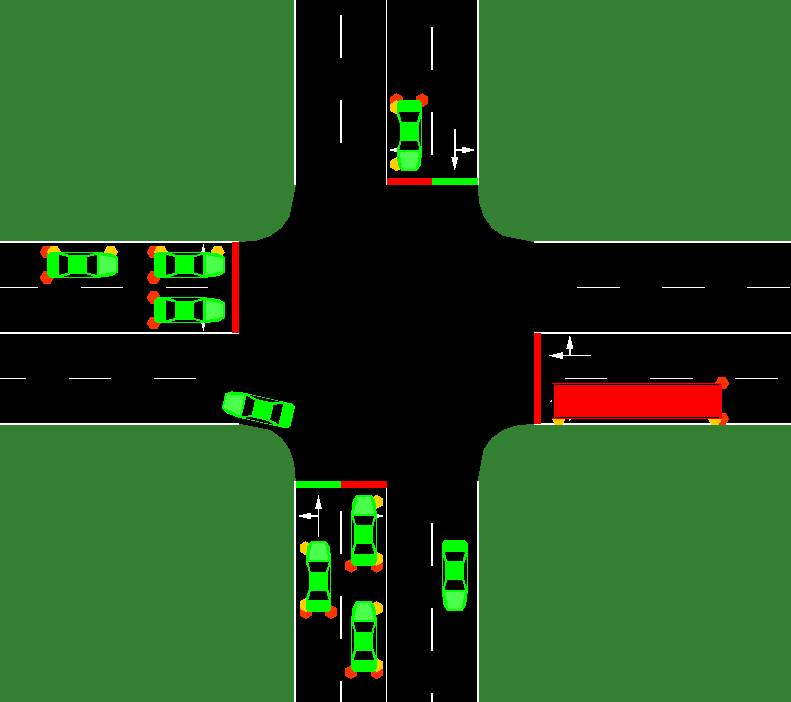
\includegraphics[width=0.7\textwidth]{intersection_map.png}
    \caption{SUMO intersection layout used in this study.}
\end{figure}

\section{Mathematical MDP Formulation}
The traffic control problem is represented as a Markov Decision Process:
\[
\mathcal{M}=\langle \mathcal{S},\mathcal{A},\mathcal{P},\mathcal{R},\gamma \rangle.
\]

\subsection{State Space}
The state vector at time step $t$ is:
\[
S_t = [Q_{NS}, Q_{EW}, W_{NS}, W_{EW}, P, T_{elapsed}].
\]
Here, $Q_{NS}$ and $Q_{EW}$ are directional queue lengths, $W_{NS}$ and $W_{EW}$ are directional waiting-time aggregates, $P$ is the active phase index, and $T_{elapsed}$ is elapsed time in the current phase.

\subsection{Action Space}
The discrete action set is defined as:
\[
A = \{0,1,2,3,4\}.
\]
Each action corresponds to a valid phase hold or phase transition in the controller.

\subsection{Reward Function}
The step reward is defined by a weighted sum of key traffic metrics:
\[
R_t = -w_1\,\Delta W_t - w_2\,Q_t - w_3\,C_t + w_4\,T_t.
\]
This multi-objective reward penalizes waiting-time growth ($\Delta W_t$), queue accumulation ($Q_t$), and switching overhead ($C_t$), while rewarding vehicle throughput ($T_t$). The optimal values for these weights ($w_1, w_2, w_3, w_4$) will be determined via a systematic ablation study in the subsequent section.

\section{Reward Function Optimization (Ablation Study)}
Before scaling the experiments to 300 episodes, an ablation study was conducted to determine the optimal configuration of the reward function weights. Ten distinct reward scenarios were evaluated by training a Q-Learning agent for 50 episodes to find the most balanced rewards.

\begin{table}[H]
\centering
\caption{Reward Function Ablation Study Summary (50 Episodes)}
\begin{tabular}{lccc}
\toprule
\textbf{Scenario Name} & \textbf{Eval Reward} & \textbf{Avg Queue} & \textbf{Avg Throughput} \\
\midrule
Baseline (0.5, 0.3, 2.0, 1.0) & -1608.30 & 11.97 & 183.00 \\
Equal Penalties & -1948.80 & 11.84 & 206.00 \\
Queue Focused & -3513.00 & 11.40 & 194.00 \\
\textbf{Wait Focused (Optimal)} & \textbf{-1144.80} & \textbf{11.80} & \textbf{217.00} \\
Strict Switch & -1751.10 & 11.32 & 193.00 \\
Lenient Switch & -1329.00 & 11.32 & 205.00 \\
High Throughput & -1384.20 & 11.75 & 197.00 \\
Low Throughput & -1606.30 & 11.42 & 183.00 \\
Balanced Aggressive & -2280.00 & 11.59 & 208.00 \\
Wait Heavy, Strict Switch & -2064.10 & 12.09 & 202.00 \\
\bottomrule
\end{tabular}
\end{table}

Based on the ablation study results, Scenario 4 (Wait Focused) provided the optimal balance by achieving the highest throughput (217.0) and the lowest penalty (-1144.80). Therefore, the final implemented reward function across all our models is:
\[
R_t = -0.8\,\Delta W_t - 0.2\,Q_t - 2.0\,C_t + 1.0\,T_t.
\]

\section{Control Strategies}

\newpage
\subsection{Fixed-Time Controller (Baseline)}
The fixed-time controller is a non-learning periodic policy that cycles through four signal phases with a green duration of 30 seconds per phase. If $k_t$ denotes elapsed steps in the current phase and $K$ is the fixed phase length (in control steps), the baseline policy can be summarized as:
\[
a_t=
\begin{cases}
0, & k_t < K,\\
\pi_{next}, & k_t \ge K,
\end{cases}
\]
where $a_t=0$ denotes keeping the current phase and $\pi_{next}$ denotes transition to the next phase in a cyclic order. While simple to implement and robust, this non-adaptive approach inevitably leads to inefficiencies during fluctuating traffic demands, as it cannot extend green lights for heavily congested lanes or skip empty ones.

\begin{figure}[H]
    \centering
    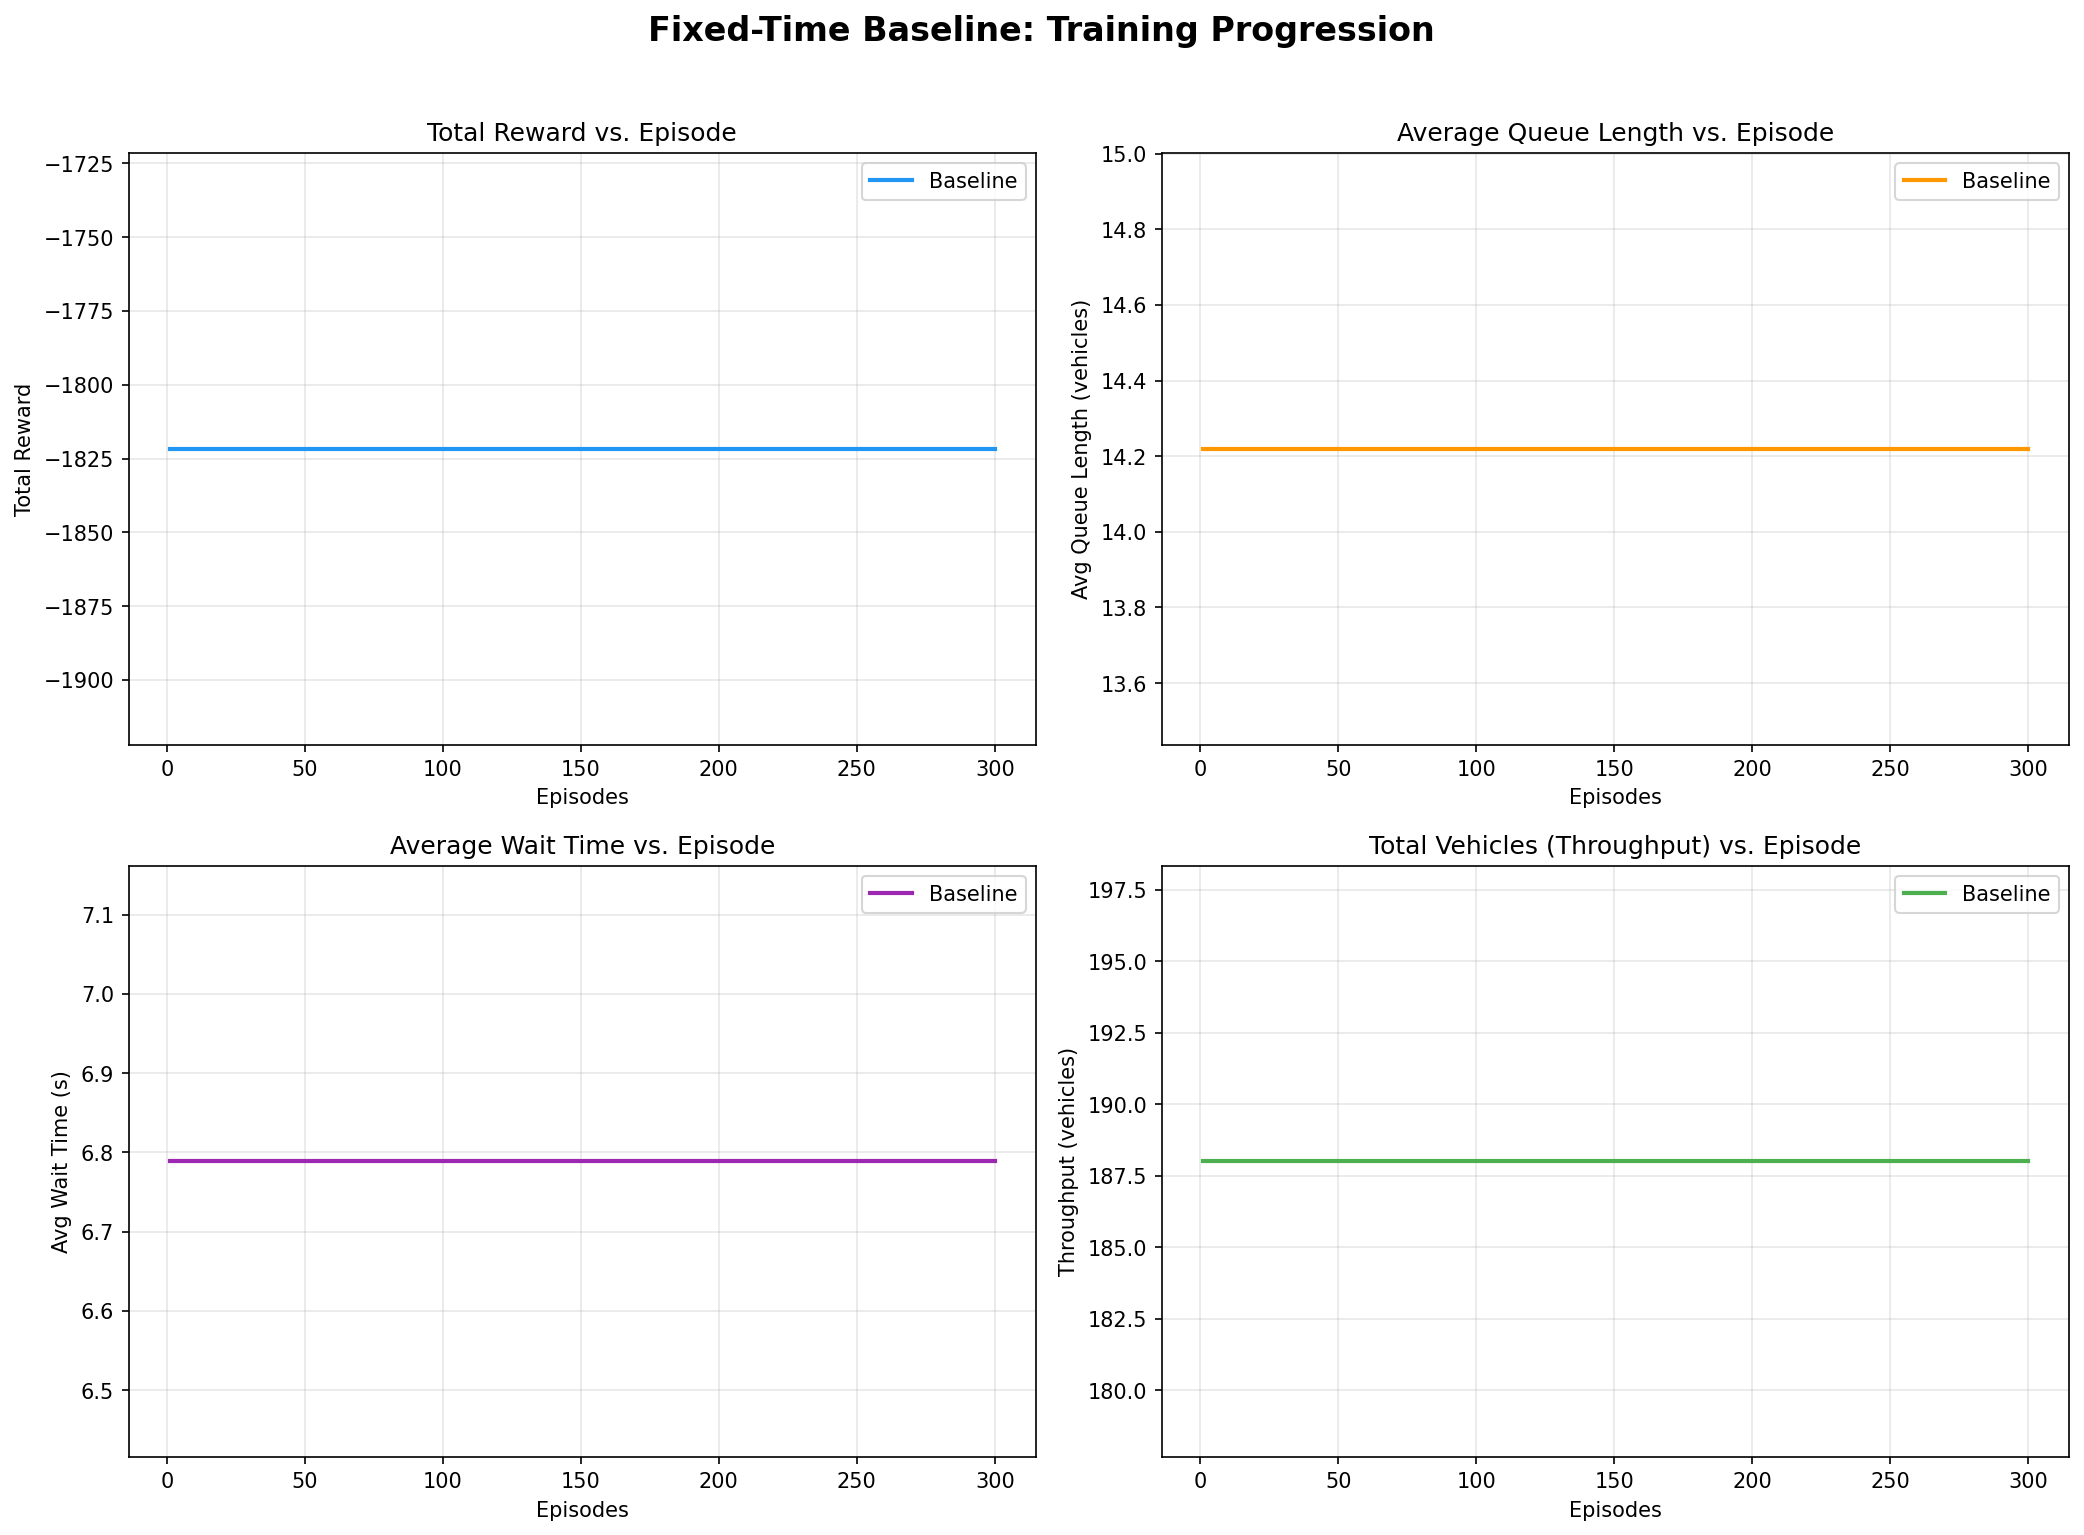
\includegraphics[width=0.8\textwidth]{fixed_time_training.png}
    \caption{Fixed-Time baseline trend over episodes.}
\end{figure}

\newpage
\subsection{Q-Learning}
Q-Learning is a foundational model-free, value-based algorithm that updates action-value estimates via temporal-difference learning. The core update rule is:
\[
Q(s_t,a_t) \leftarrow Q(s_t,a_t) + \alpha\left[r_t + \gamma\max_{a'}Q(s_{t+1},a') - Q(s_t,a_t)\right].
\]
The policy is typically implemented with $\epsilon$-greedy exploration during training. However, standard Q-learning suffers from an \textbf{Overestimation Bias} because the maximization step ($\max_{a'}Q(s_{t+1},a')$) uses the same values to both select and evaluate an action. In stochastic environments like traffic control, this can lead to overly optimistic value estimates that degrade the final policy's performance.

\begin{figure}[H]
    \centering
    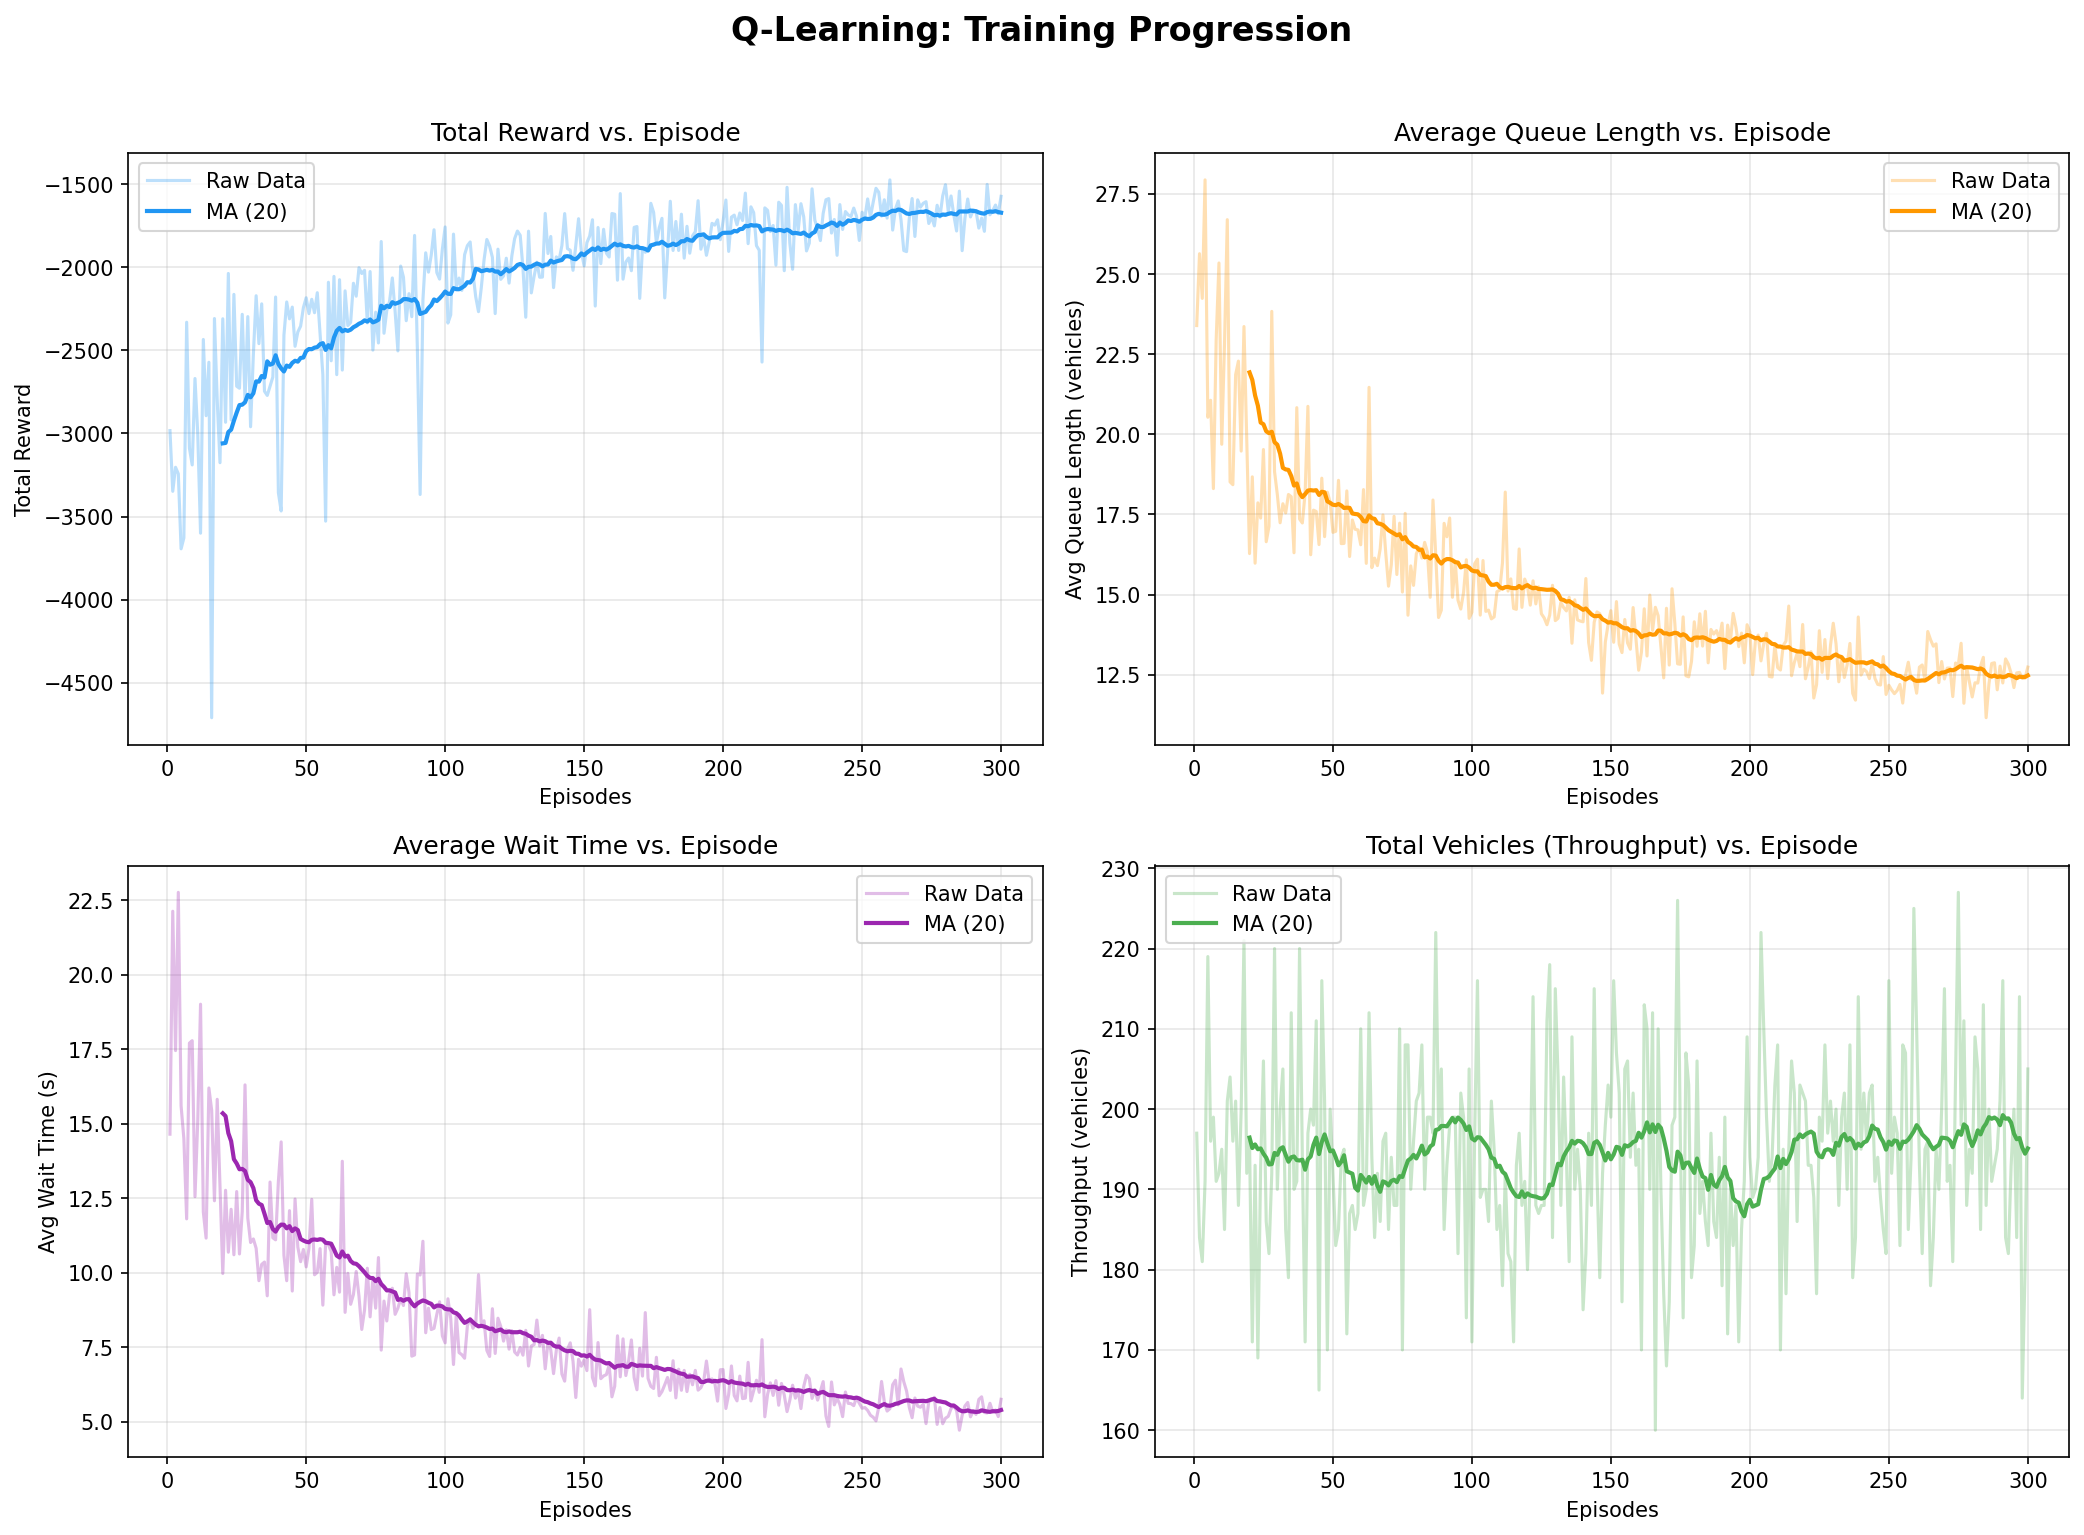
\includegraphics[width=0.8\textwidth]{q_learning_training.png}
    \caption{Q-Learning training progression.}
\end{figure}

\newpage
\subsection{Double Q-Learning}
Double Q-Learning explicitly solves the overestimation bias inherent in standard Q-Learning by decoupling the action selection from the action evaluation. It maintains two separate value functions (or tables), $Q^A$ and $Q^B$. When updating $Q^A$, the algorithm uses $Q^A$ to select the best next action, but uses $Q^B$ to evaluate that action's value:
\[
Q^A(s_t,a_t) \leftarrow Q^A(s_t,a_t) + \alpha\left[r_t + \gamma Q^B\left(s_{t+1},\arg\max_{a'}Q^A(s_{t+1},a')\right) - Q^A(s_t,a_t)\right].
\]
The symmetric counterpart is obtained by swapping $A$ and $B$. By untangling selection and evaluation, Double Q-Learning provides much more stable and realistic value estimations, leading to significantly better long-term routing decisions.

\begin{figure}[H]
    \centering
    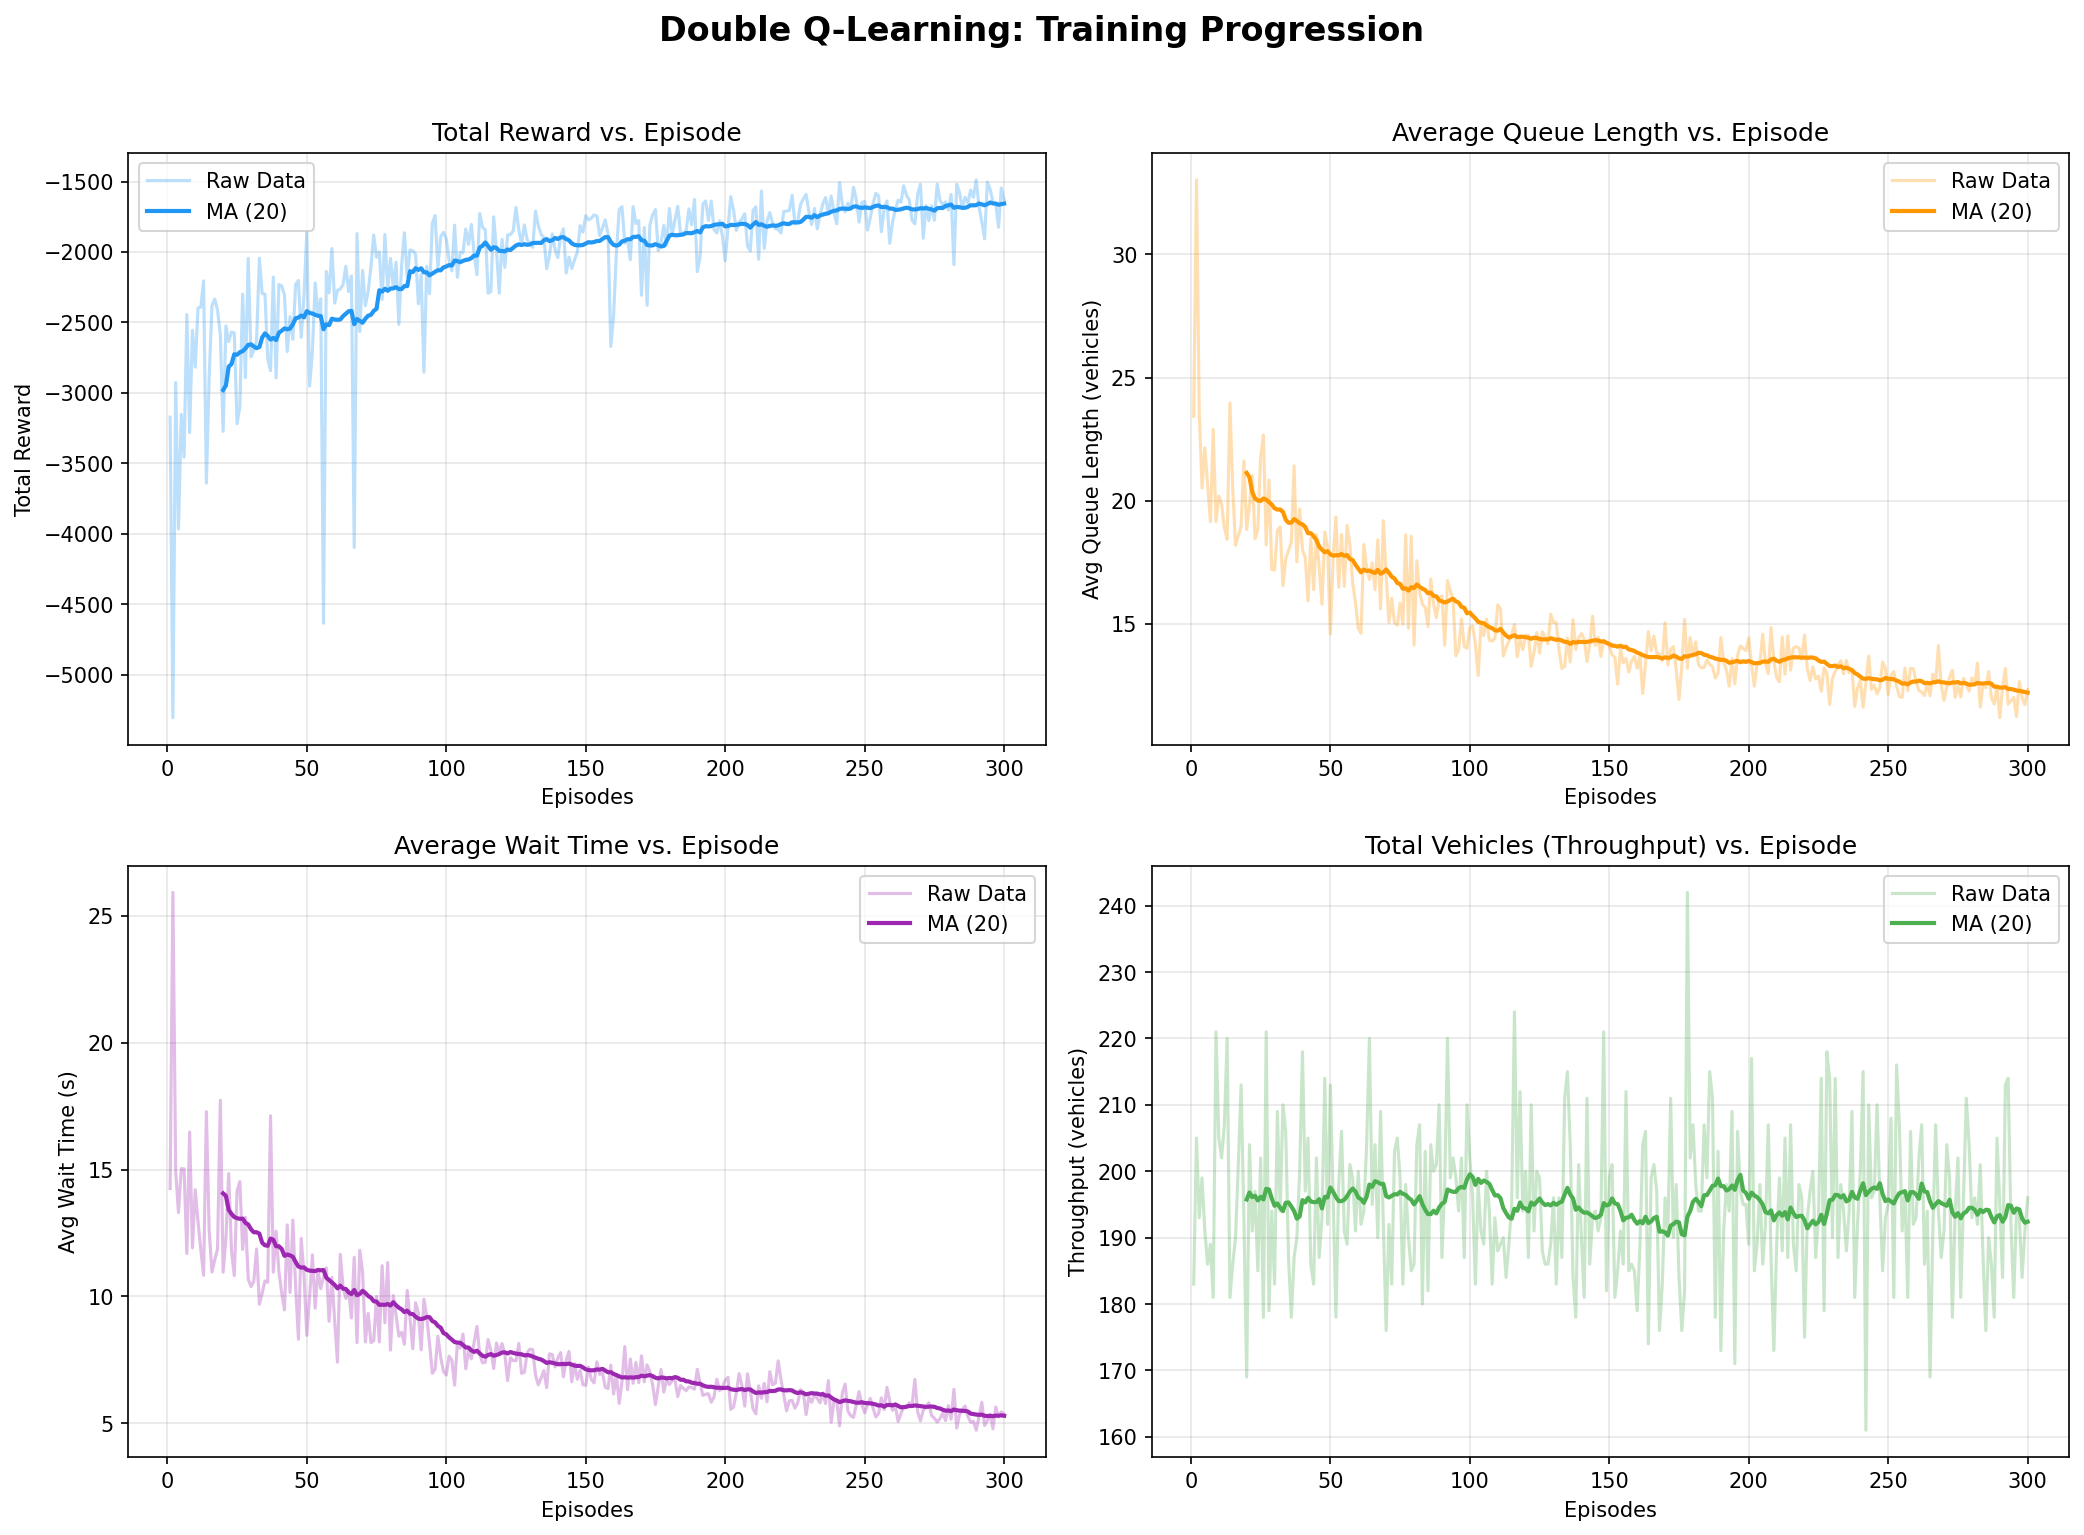
\includegraphics[width=0.8\textwidth]{double_q_training.png}
    \caption{Double Q-Learning training progression.}
\end{figure}

\newpage
\subsection{Deep Q-Network (DQN)}
DQN transitions from tabular methods to deep reinforcement learning by approximating the action-value function $Q(s,a;\theta)$ using a neural network. To stabilize training, DQN introduces two critical components: a \textbf{Replay Buffer} and a \textbf{Target Network}. The replay buffer stores past experiences $(s, a, r, s')$ and samples them randomly during training, which breaks the temporal correlation between consecutive traffic states. The target network ($\theta^-$) provides stable temporal-difference targets:
\[
y_t = r_t + \gamma\max_{a'}Q(s_{t+1},a';\theta^-).
\]
Using Huber loss for robustness against outliers, the objective is:
\[
\mathcal{L}(\theta)=\mathbb{E}_{(s,a,r,s')\sim\mathcal{D}}\left[\ell_\delta\left(y_t - Q(s_t,a_t;\theta)\right)\right].
\]

\begin{figure}[H]
    \centering
    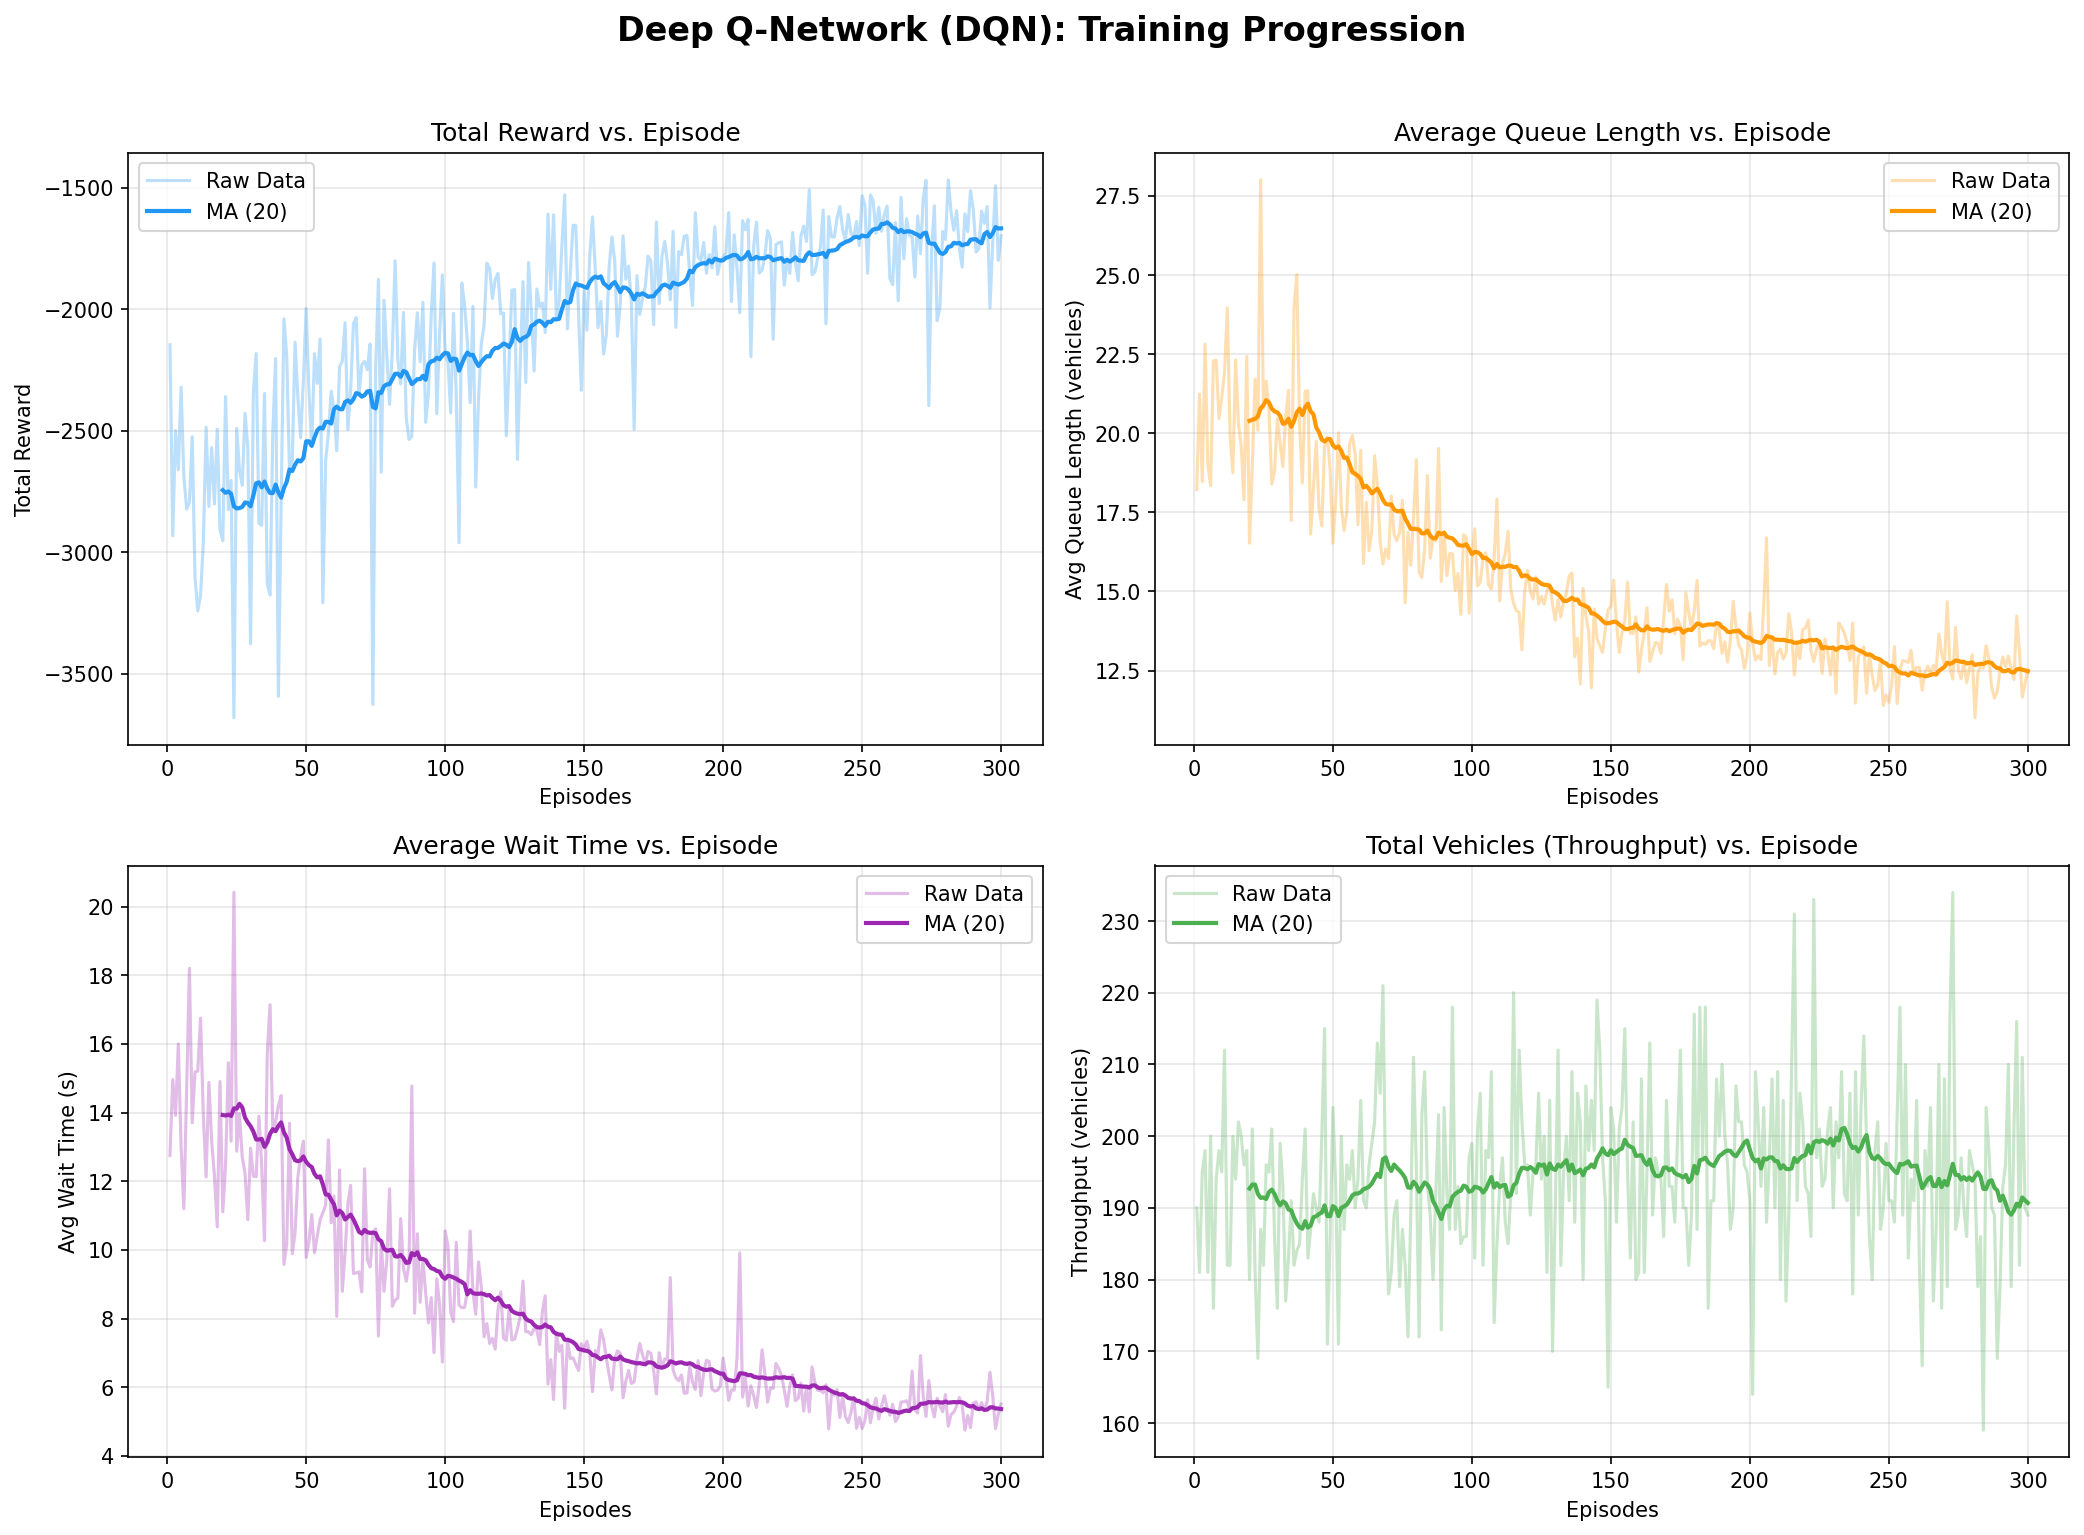
\includegraphics[width=0.8\textwidth]{dqn_training.png}
    \caption{DQN training progression.}
\end{figure}

\newpage
\subsection{Advantage Actor-Critic (A2C)}
A2C is a hybrid Policy Gradient algorithm that utilizes two separate neural networks: an \textbf{Actor} and a \textbf{Critic}. The Actor parameterizes the policy $\pi(a|s;\theta)$ to directly select actions, while the Critic estimates the value function $V(s;\phi)$ to evaluate how good a state is. Updates are driven by the \textbf{Advantage function}:
\[
A(s_t, a_t) = Q(s_t, a_t) - V(s_t) \approx r_t + \gamma V(s_{t+1}) - V(s_t).
\]
The Advantage function measures how much better an action was compared to the average expected reward of that state. By using the Advantage rather than raw returns, A2C significantly reduces the high variance typically associated with standard policy gradient updates:
\[
\nabla_\theta J(\theta) \approx \mathbb{E}\left[ \nabla_\theta \log \pi(a_t|s_t;\theta) A(s_t, a_t) \right].
\]

\begin{figure}[H]
    \centering
    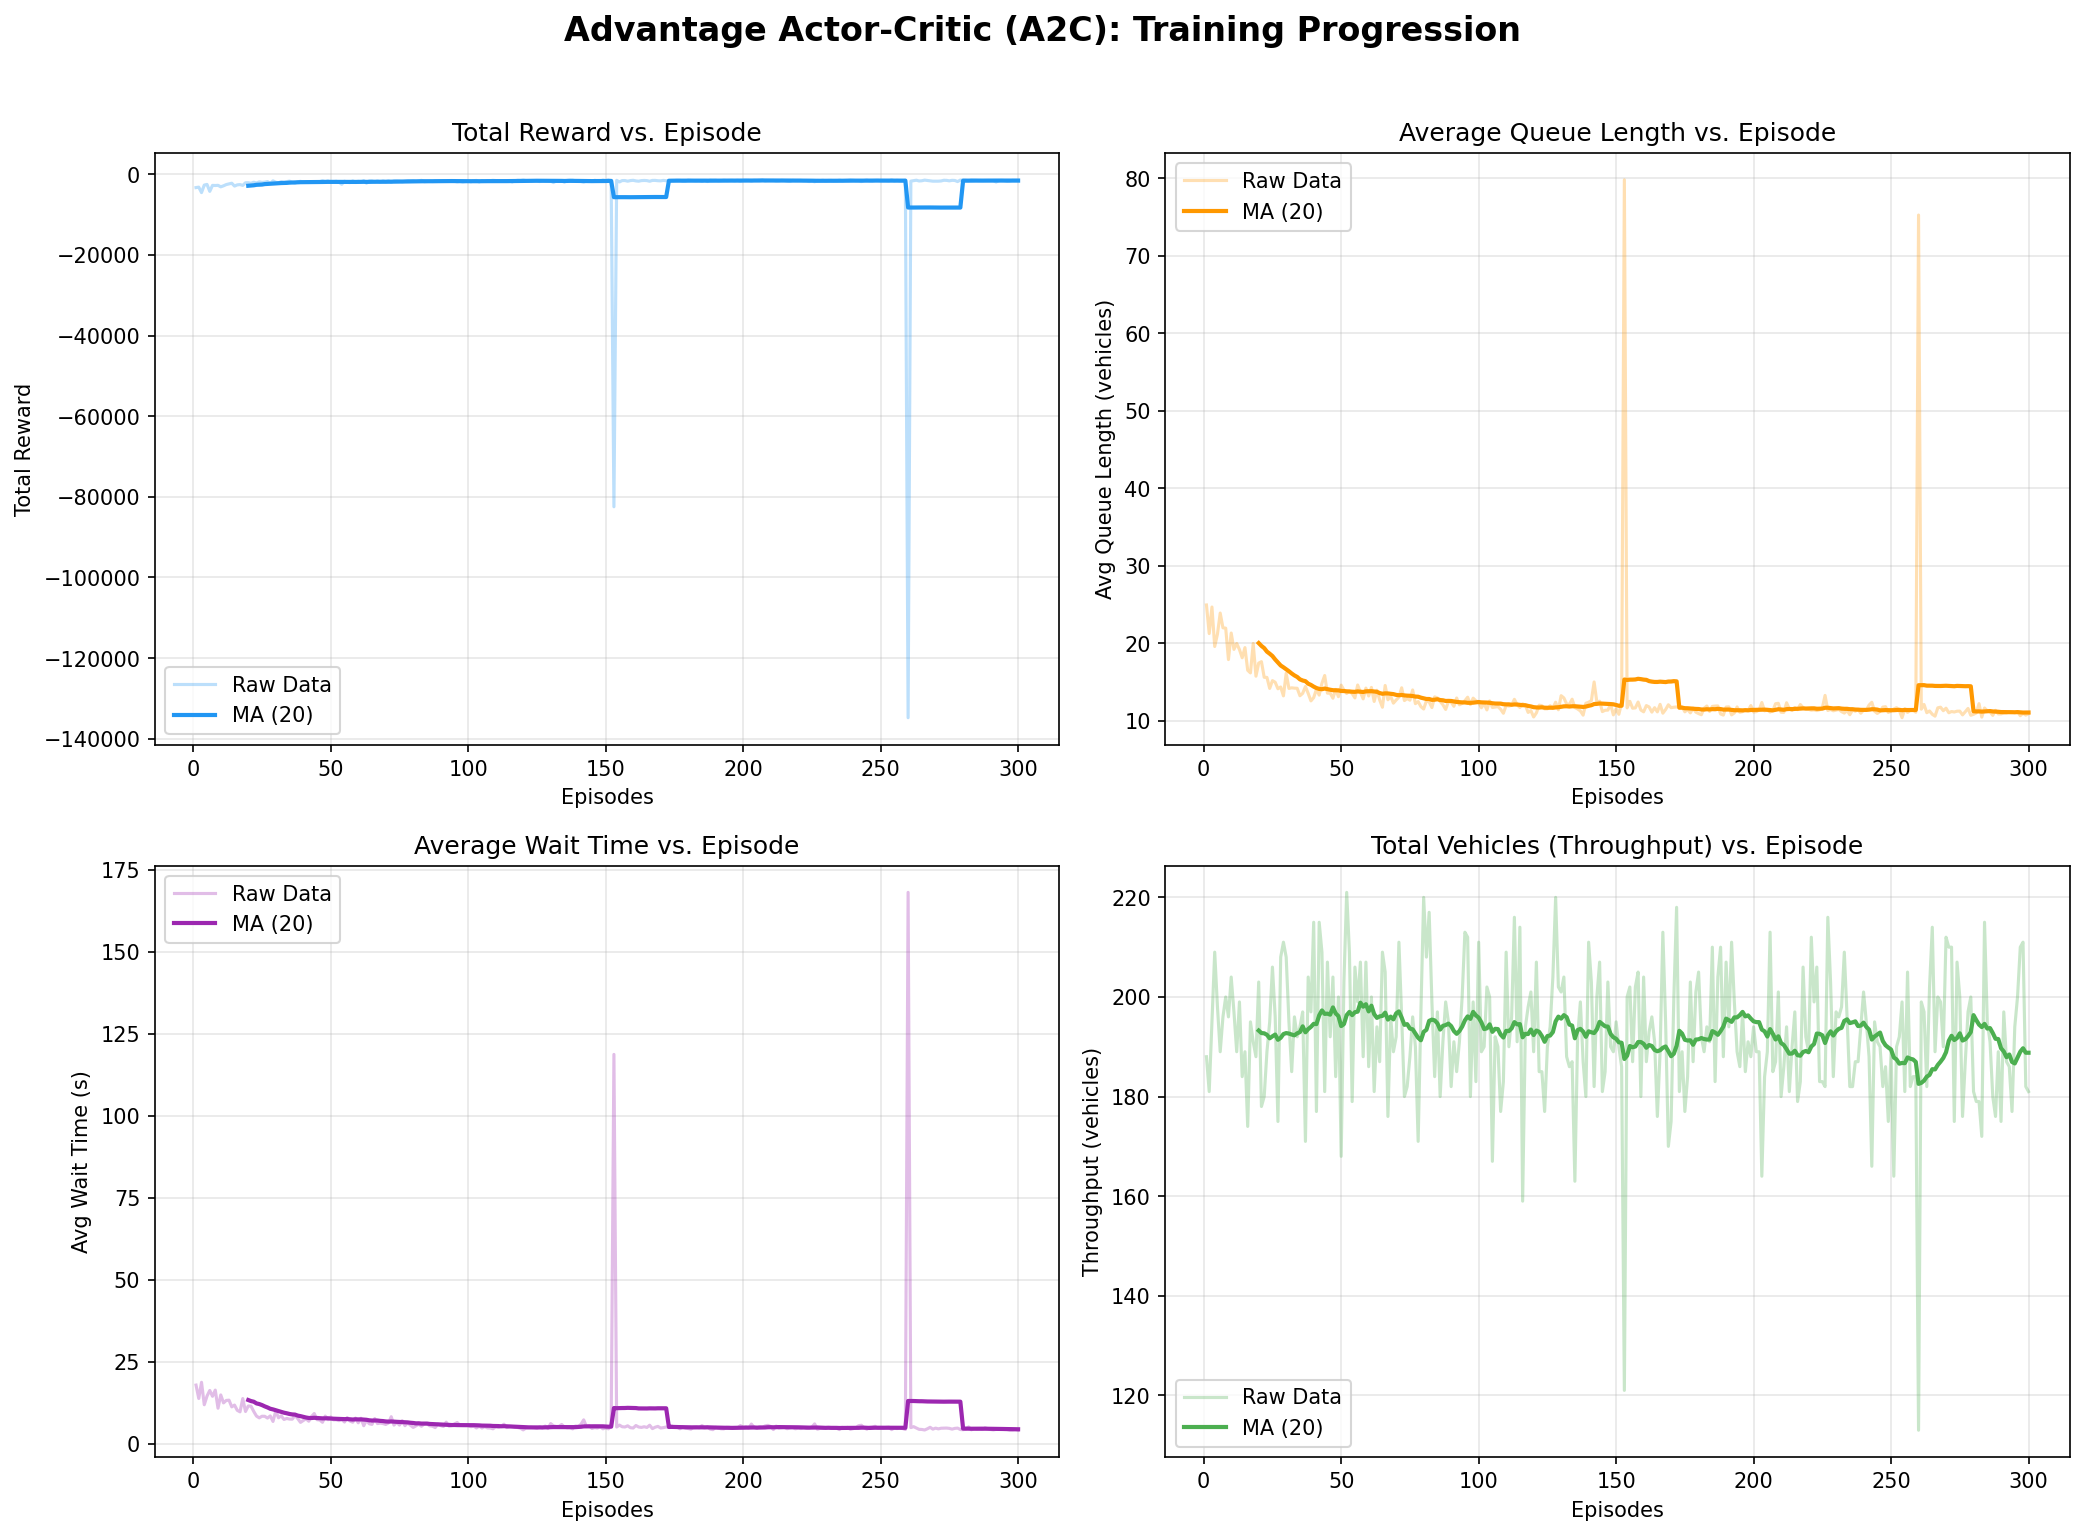
\includegraphics[width=0.8\textwidth]{a2c_training.png}
    \caption{A2C training progression.}
\end{figure}

\newpage
\subsection{Proximal Policy Optimization (PPO)}
PPO improves upon standard policy gradients by preventing destructively large policy updates that can collapse the agent's learning progress. It optimizes a \textbf{Clipped Surrogate Objective} using a probability ratio $r_t(\theta) = \frac{\pi_\theta(a_t|s_t)}{\pi_{\theta_{old}}(a_t|s_t)}$. The clipping mechanism ensures that the new policy does not deviate too far from the old policy:
\[
L^{CLIP}(\theta) = \mathbb{E}\left[ \min\left( r_t(\theta)A_t, \text{clip}(r_t(\theta), 1-\epsilon, 1+\epsilon) A_t \right) \right].
\]
By dynamically bounding the policy updates within the $[1-\epsilon, 1+\epsilon]$ range, PPO guarantees stable, monotonic learning steps without the complex second-order mathematics required by earlier algorithms.

\begin{figure}[H]
    \centering
    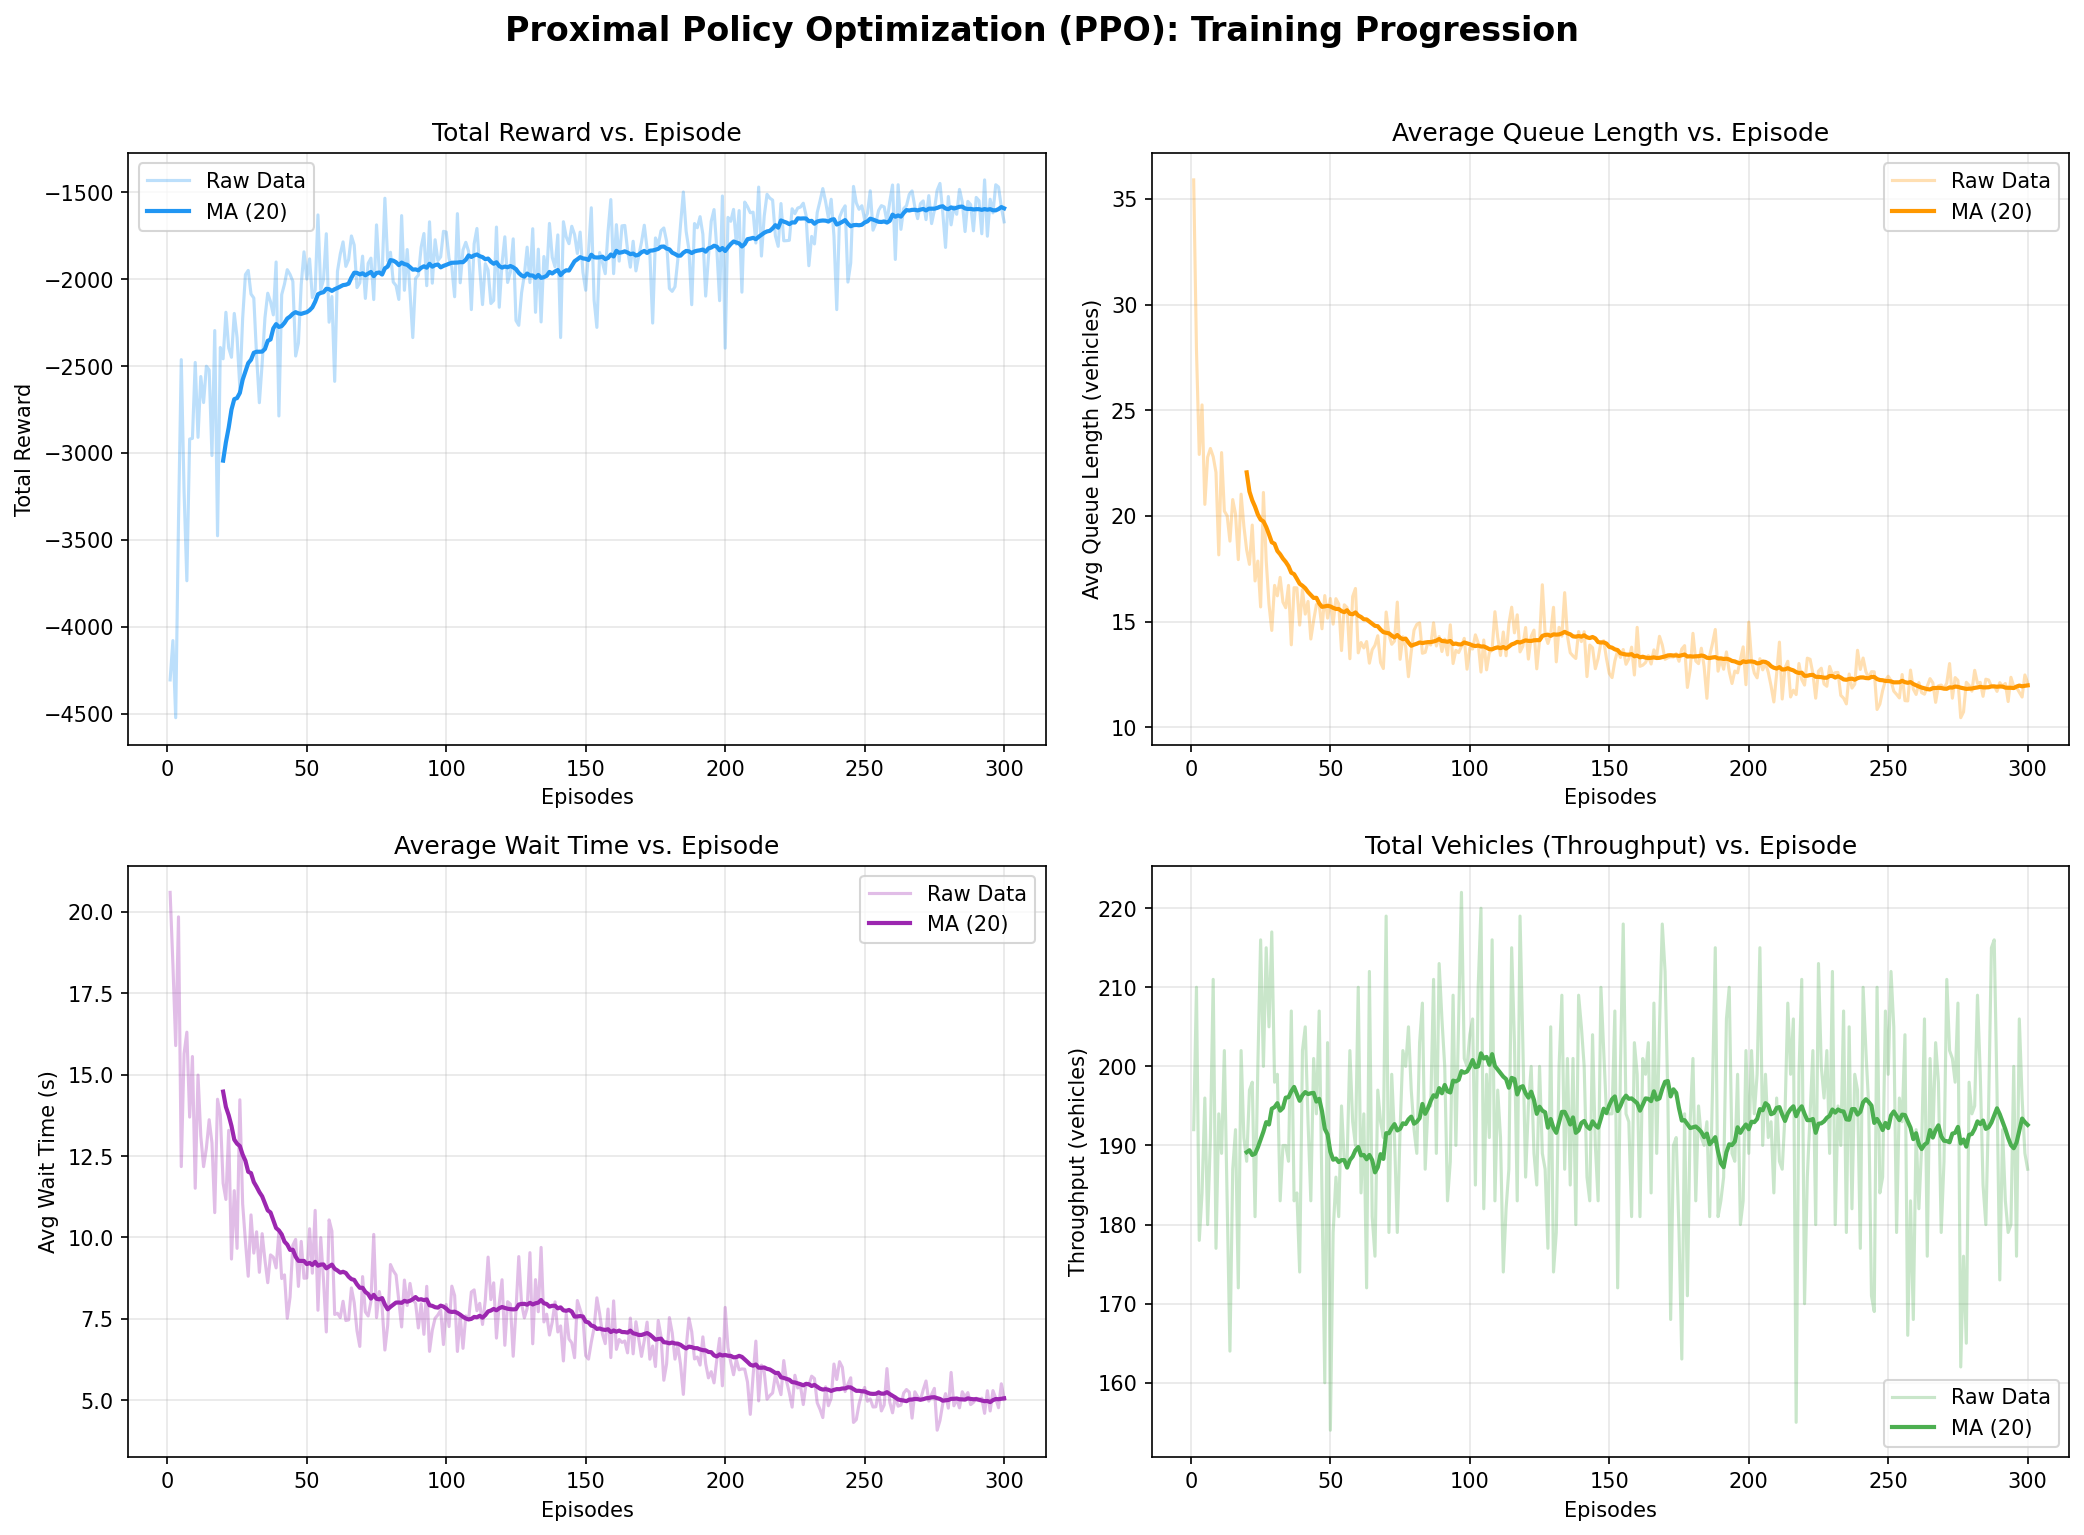
\includegraphics[width=0.8\textwidth]{ppo_training.png}
    \caption{PPO training progression.}
\end{figure}

\newpage
\subsection{Trust Region Policy Optimization (TRPO)}
TRPO theoretically guarantees monotonic policy improvement by enforcing a hard \textbf{Trust Region} constraint on the Kullback-Leibler (KL) divergence between the old and new policies. Rather than clipping like PPO, TRPO solves a constrained optimization problem to ensure the policy strictly stays within a safe neighborhood:
\[
\max_\theta \mathbb{E}\left[ \frac{\pi_\theta(a_t|s_t)}{\pi_{\theta_{old}}(a_t|s_t)} A_t \right] \quad \text{subject to} \quad \mathbb{E}\left[ D_{KL}(\pi_{\theta_{old}} || \pi_\theta) \right] \le \delta.
\]
While this rigorous mathematical constraint makes TRPO exceptionally safe and stable—preventing catastrophic forgetting in complex environments—it is significantly more computationally expensive to calculate the Fisher Information Matrix than standard first-order policy gradients.

\begin{figure}[H]
    \centering
    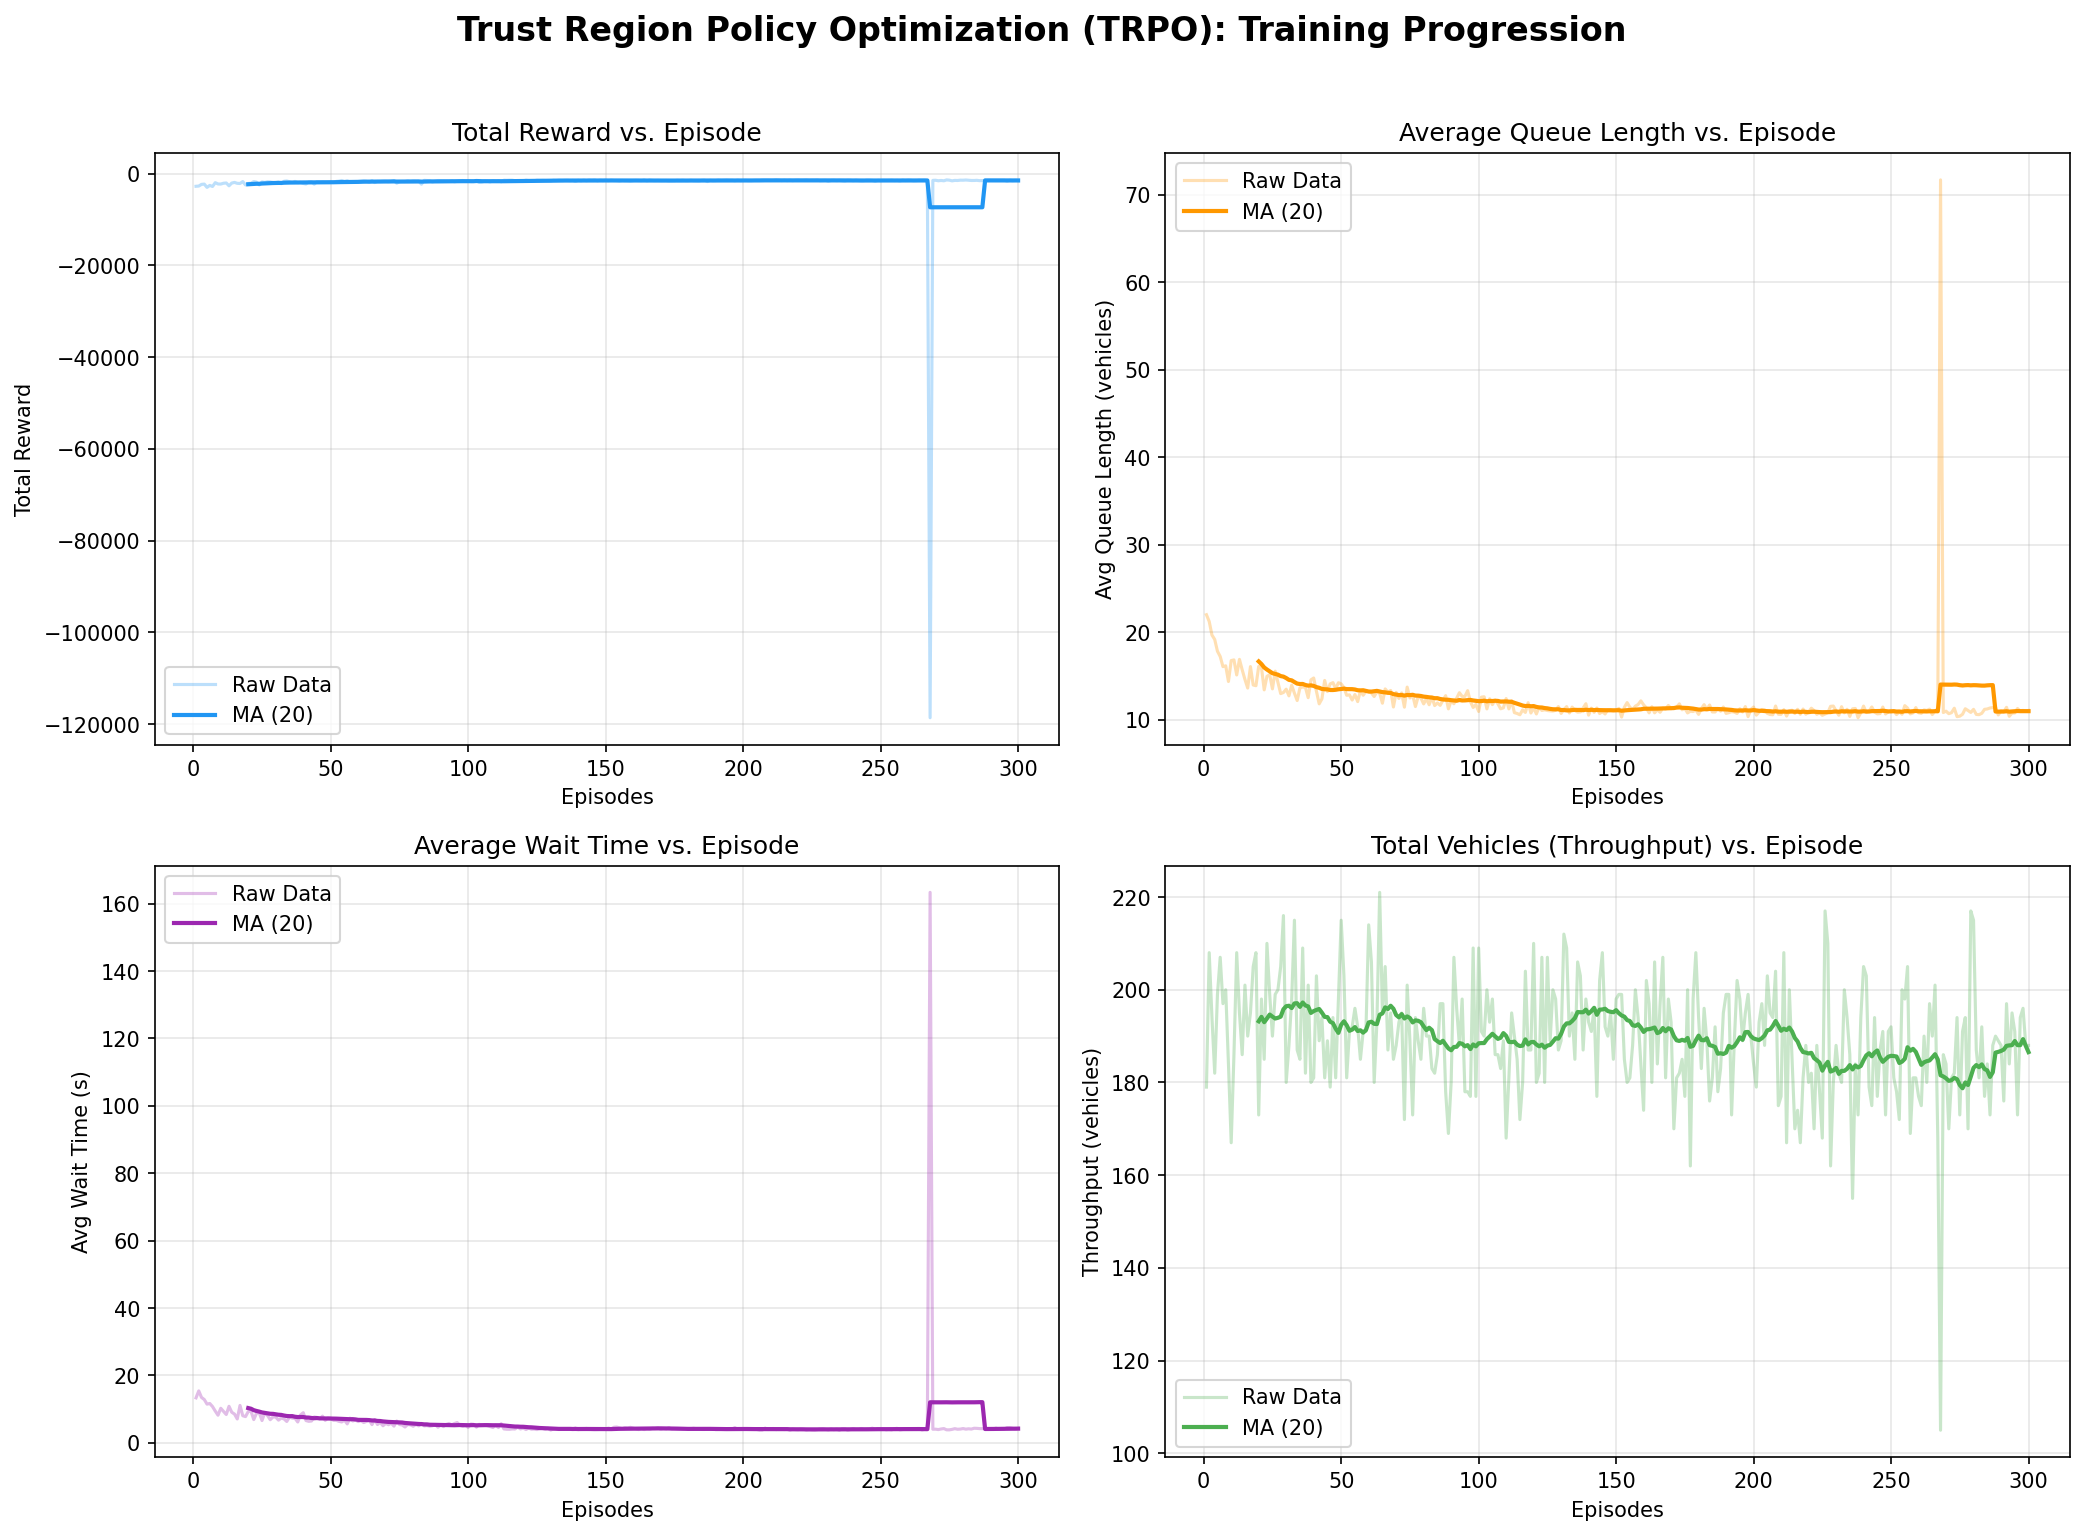
\includegraphics[width=0.8\textwidth]{trpo_training.png}
    \caption{TRPO training progression.}
\end{figure}

\newpage
\section{Experimental Results}
\begin{figure}[H]
    \centering
    
\includegraphics[width=0.8\textwidth]{training_convergence.png}
    \caption{Overall convergence comparison across all controllers.}
\end{figure}

\begin{table}[H]
\centering
\caption{Final Performance Metrics Comparison across all Agents}
\begin{tabular}{lccccc}
\toprule
\textbf{Agent} & \textbf{Avg Queue} & \textbf{Wait (s)} & \textbf{Throughput} & \textbf{Delay (s)} & \textbf{Avg Reward} \\
\midrule
Fixed-Time & 14.22 & 6.79 & 188.0 & 8.92 & -1821.70 \\
Q-Learning & 11.71 & 4.47 & 191.0 & 6.72 & -1636.60 \\
\textbf{Double Q-Learning} & \textbf{11.11} & 4.57 & \textbf{200.0} & 6.81 & \textbf{-1427.50} \\
DQN & 12.45 & 5.08 & 190.7 & 7.29 & -1720.90 \\
A2C & 11.40 & 4.53 & 175.3 & 6.83 & -1540.70 \\
PPO & 12.04 & 5.05 & 184.0 & 7.30 & -1625.20 \\
\textbf{TRPO} & 11.18 & \textbf{4.26} & 182.0 & \textbf{6.55} & -1571.10 \\
\bottomrule
\end{tabular}
\end{table}

\begin{figure}[H]
    \centering
    
\includegraphics[width=0.8\textwidth]{metric_comparison_bars.png}
    \caption{Final metric comparison among all methods.}
\end{figure}

\subsection{Discussion of Results}

The extended 300-episode results definitively demonstrate that adaptive Reinforcement Learning policies significantly outperform the traditional Fixed-Time baseline across all critical traffic metrics. However, analyzing the performance of the various agents reveals a profound \textbf{Efficiency Trade-off} between Value-based and Policy Gradient methodologies. Double Q-Learning achieved the absolute highest \textbf{Throughput (200.0 vehicles)}, operating on the principle of quantity. In contrast, TRPO successfully optimized the quality of the traffic flow, achieving the lowest \textbf{Average Wait Time (4.26s)} and \textbf{Average Delay (6.55s)}. This dichotomy suggests that Value-based methods aggressively prioritize flushing large clusters of vehicles through the intersection to maximize reward, whereas Policy Gradient methods develop highly nuanced, micro-level timing strategies to prevent individual vehicles from stalling, ultimately minimizing overall delay.

A critical factor in the success of the Deep RL agents (DQN, A2C, PPO, TRPO) was the \textbf{Impact of State Normalization}. In urban traffic environments, variables such as accumulated waiting time can easily exceed values of 1000+, whereas active phase indices remain strictly bounded between 0 and 3. Without robust normalization, these massive unscaled inputs cause catastrophic gradient explosions within neural networks. Implementing an online running mean and standard deviation scaler (Welford's algorithm) was crucial for stabilizing the neural policies, allowing complex algorithms like PPO and TRPO to converge efficiently over the 300-episode span.

Finally, an analysis of the \textbf{Tabular vs. Deep RL} performance reveals a fascinating dynamic regarding the curse of dimensionality. Despite the sophisticated architectures of neural networks, tabular methods like Double Q-Learning remain highly competitive---and often superior---in this specific environment. Because our state space was strictly macroscopic and highly compact (a 6D continuous vector), the tabular discretization was able to map the state-action space efficiently without suffering from memory constraints. Deep RL networks inherently carry high computational overhead and require massive amounts of data to break correlations and learn optimal representations. Consequently, in mathematically dense but dimensionally small environments, the direct action-value mapping of tabular Double Q-Learning proved to be the most sample-efficient and robust approach for maximizing sheer traffic throughput.

\section{Conclusion}
This report demonstrates the effectiveness of Reinforcement Learning for adaptive urban signal control under a realistic SUMO-based setup. Relative to the Fixed-Time baseline, all RL methods markedly improve traffic flow efficiency. Importantly, the expanded 300-episode experiments highlighted a core trade-off in control strategies: Value-based methods, specifically Double Q-Learning, are superior for raw throughput optimization, whereas advanced Policy Gradient methods, notably TRPO, excel at precisely minimizing wait times and delays. These findings provide strong empirical support for the deployment of specialized, learning-based controllers tailored to specific traffic management priorities.

\end{document}